\documentclass[master,english]{hgbthesis}
% Zulässige Class Options: 
%   Typ der Arbeit: diplom, master (default), bachelor, praktikum 
%   Hauptsprache: german (default), english
%%------------------------------------------------------------

% packages
\usepackage{pgfplots}
\usepackage{tikz}
\usepackage{color}
\usepackage{enumitem}
\usepackage{multicol}

% root folder of OMNeT++ installation
\newcommand{\omnetpproot}{/opt/omnetpp-4.6}

% lstintputlistings style
\definecolor{xCodeComment}{RGB}{0,143,0}
\definecolor{xCodeWordStyle}{RGB}{216,33,174}
\definecolor{xCodeStringStyle}{RGB}{235,0,65}
\definecolor{xCodePreprocessor}{RGB}{130,71,33}
\definecolor{LightGray}{RGB}{240,240,240}

\lstset{language=C++,
    numbers=left,
    numberstyle=\tiny,
    basicstyle =\ttfamily\fontsize{8}{10}\selectfont,
    keywordstyle =\color{xCodeWordStyle},
    commentstyle = \color{xCodeComment},
    stringstyle = \color{xCodeStringStyle},
    showstringspaces = true,
    backgroundcolor=\color{white},
    framexrightmargin=2mm,
    breaklines=true,
    emph={\#endif},
    emphstyle={\color{xCodePreprocessor}},
    caption=\lstname,
    inputencoding={utf8},
    extendedchars=false
}



\graphicspath{{images/}}    % name of directory containing the images
\logofile{FHOOeIntl2014}	% name of PDF, remove or use \logofile{} for no logo
\bibliography{literature}  	% name of the BibTeX (.bib) file

% disable colored borders for hyperlinks
%\hypersetup{
%    colorlinks=false,
%    pdfborder={0 0 0},
%}

%%%----------------------------------------------------------
\begin{document}
%%%----------------------------------------------------------

% Einträge für ALLE Arbeiten: --------------------------------
\title{Simulation and emulation of realtime communication networks}
\author{Franz Profelt}
\studiengang{Embedded Systems Design}
\studienort{Hagenberg}
\abgabedatum{2016}{05}{20}	% {YYYY}{MM}{DD}

%%% zusätzlich für eine Bachelorarbeit: ---------------------
\nummer{XXXXXXXXXX-A}   % XX...X = Stud-ID, z.B. 0310238045-A  
                        % (A = 1. Bachelorarbeit)
\semester{Sommersemester 2012} 
\gegenstand{Einführung in die Tiefere Problematik 1} 
\betreuer{Alois B.~Treuer, Päd.\ Phil.} % oder \betreuerin{..}

%%% zusätzlich für einen Praktikumsbericht: -----------------
\nummer{XXXXXXXXXX-B}   % XX...X = Stud-ID, z.B. 0310238045-B  
                        % (B = 2. Bachelorarbeit)
\betreuer{Mag.~Pjotr I.~Czar\\Creative Director}  % \betreuerin{..}
\firma{%
   Oligarchic Media International GmbH\\
   Online Division\\
   1020 Wien, Hubertusgasse 3a
}
\firmenTel{1-234-5678-100}
\firmenUrl{www.mogul.at}

%\strictlicense  % erzeugt restriktive Lizenzformel

%%%----------------------------------------------------------
\frontmatter
\maketitle
\tableofcontents
%%%----------------------------------------------------------

\chapter{Abstract}

%TODO: (re)write abstract

% imported from paper
OMNeT++ embodies a framework for simulations. This includes different functionalities for communication in between modules and components written in C++.
The normal simulation using OMNeT++ is event based and is achieved independent of the real time.

OMNeT++ provides the possibility for running a simulation in real time i.e. every simulated second is processed within a real second.
Such a real time simulation attempts to process the simulation with real world timings and delays.
The possibility to run simulated software with real timings allows the field of emulation and the connection of simulated components with real hardware or software.
Such a real time simulation and its limits regarding possible timings depends on the used host system.
Implementing the simulation for a given software system using OMNeT++ can be achieved with different designs and various numbers of modules and transmitted messages.
These factors will impact the efficiency of the real time simulation and achieved timings.

This paper investigates the functionality of OMNeT++ regarding simulation and real time simulation.

%TODO: write german abstract			
% !TeX spellcheck = de_AT_frami

\chapter{Kurzfassung}
\begin{german}
Die Themengebiete der Simulation und Emulation gewinnen stetig an Bedeutung für die Entwicklung von eingebetteten Systemen.
Dies wird verursacht durch die steigende Nachfrage nach umfangreichen Tests.
Eine Vielzahl von Anwendungsgebieten erfordern einen hohen Grad an Testungen.

Dieser Trend führt zu einem steigendem Interesse an der Entwicklung einer Simulation oder Emulation für bestehende oder neu entwickelte Systeme.
Es existiert eine große Anzahl von verschiedenen Systemen zur Entwicklung von Simulationen die oftmals vielseitige Konfigurationsmöglichkeiten bieten.
Dieser Überfluss an verschiedenen Möglichkeiten eine Simulation zu entwickeln, kann Entwickler von der Entscheidung abhalten, eine Simulation für ihren Nutzen zu entwickeln.
OMNeT++ stellt ein sehr flexibles System zur Entwicklung von Simulationen für verschiedenste Anwendungen dar.

\begin{sloppypar}
Diese Arbeit analysiert den Aufbau und die Eigenschaften von OMNeT++ und zeigt die Möglichkeiten zur Konfiguration und Anpassung auf.
Es werden unterschiedliche Leistungsmessungen durchgeführt, die eine Testsimulation im Bezug auf Laufzeit, verarbeiteten Ereignissen und Echtzeiteigenschaften überprüft.
Es wurde ein optimierter Aufbau der Simulation gefunden, welcher zu einem verbesserten Ergebnis der Leistung führt.
Die vorhandenen Funktionen und die Möglichkeiten zur Entwicklung einer Echtzeitsimulation und Emulation stellt eine interessante Methode zum Testen und Entwickeln von eingebetteten Systemen dar.
Die Open Source Implementierung openPOWERLINK bietet die Möglichkeit, ein bestehendes Echtzeitkommunikationssystem zu analysieren und für eine Simulation anzupassen.
openPOWERLINK implementiert das weit verbreitete POWERLINK Protokoll um, welches häufig im Bereich der Industrieautomation und Echtzeitkommunikation eingesetzt wird.
Bei der Entwicklung einer Simulation, die ein gegebenes System, wie die openPOWERLINK Implementierung, einbindet, werden Fragen bezüglich Mehrfachinstanzen aufgeworfen.
Es wurde eine Lösung für diese Problematik gefunden und es wurde eine Simulation entwickelt, die ein aus openPOWERLINK Knoten bestehend POWERLINK Netzwerk nachstellt.
\end{sloppypar}
    
\end{german}
		

%%%----------------------------------------------------------
\mainmatter         % Hauptteil (ab hier arab. Seitenzahlen)
%%%----------------------------------------------------------

\chapter{Introduction}
\label{cha:introduction}
This thesis is intended to analyze the simulation framework \emph{OMNeT++} \cite{omnet_manual} and the possibilities for real-time simulation and emulation of a real-time communication network.
A test simulation is analyzed for determining an optimized design regarding performance and real-time capabilities.
Furthermore, a simulation of the real-time communication protocol POWERLINK and its open source implementation \mbox{openPOWERLINK} \cite{openpowerlink} is implemented. 
For developing this simulation, the openPOWERLINK stack is analyzed and the platform dependencies are investigated.

\section{Motivation}
% needs and requirements for embedded systems
The fields of embedded systems and real-time communication entail critical requirements for timings and deterministic behavior.
The development of systems meeting those requirements can be very difficult due to the lack of possibilities for sufficient testing.
A variable testing environment facilitates the development and verification of such systems.
The correct replication of complex scenarios and special operating conditions is not always possible.
Therefore the need for simulation is gaining importance with increasing complexity of embedded systems.

% real world simulation
Extended functionalities of simulation frameworks allow the usage as real-time simulation.
By simulating a system in real time, i.e. the simulated time passes according to the real (world) time, these simulations can be used in the fields of emulation and hardware in the loop (\emph{HiL}).
This allows variable testing scenarios built with a simulated environment.
These fields are necessary for testing embedded systems due to the increased possibilities of testing scenarios and setups.

Because of the raising importance of simulation and emulation. the analysis of simulation frameworks and the development of simulations for real-time communication systems represent an important field.

\section{Content}

% first chapters fundamentals and basics of OMNeT++, simulation, emulation, simulated designs, parallel simulation
Chapters \ref{cha:omnet} to \ref{cha:parallel_sim} describe fundamentals regarding OMNeT++, general simulations, emulations and \emph{HiL}, simulation designs and parallel simulation.
These chapters intend to provide an extensive introduction and preparation for further analyses.

% development of a example network for design analyze and discussion of results
Chapter \ref{cha:measurements} discusses the analysis of two different fundamental designs and their impact on the achieved performance.
This performance is measured in multiple ways to analyze the simulation regarding runtime, processed events and real-time behavior.

% fundamentals of openPOWERLINK with focus on platform dependency and porting possibilities
Subsequently, the Open Source stack openPOWERLINK is analyzed placing a special focus on the structure and the platform dependencies.
As outlined in chapter \ref{cha:oplk}, these dependencies are used for the following development of an OMNeT++ simulation embedding the openPOWERLINK stack.
% approach to simulate openPOWERLINK in OMNeT++
This simulation and the implementation strategies are discussed in chapter \ref{cha:porting}.

% conclusion
Finally the experiences and knowledge gained during this research are concluded and listed in chapter \ref{cha:conclusion}.

% appendix
The appendix contains three chapters and comprises code snippets from the OMNeT++ framework (\ref{app:omnetpp_code}), additional design measurements (\ref{app:measurements}) and some implementation samples of the openPOWERLINK simulation and the integration of the openPOWERLINK stack (\ref{app:simulation}).

\section{Purpose}
The purpose of this thesis is an analysis of the OMNeT++ framework and its capabilities regarding real-time simulation.
Furthermore it is intended to perform an analysis of the openPOWERLINK stack focusing on the platform dependencies.
This leads to the development of a simulation embedding openPOWERLINK nodes within a simulation POWERLINK network.

This thesis demonstrates the capabilities and strategies of developing a simulation for an embedded real-time communication network.
\chapter{OMNeT++}

\label{sec:OMNeT}
OMNeT++ represents a simulation framework written in C++ and is a open source project.
The commercial supported version is OMNEST and provides licensing models, whereas OMNeT++ is only available for academic or non-profit use.
The intention of OMNeT++ is providing infrastructure for writing simulations for various fields.
Especially in the field of network simulations OMNeT++ is widely used due the big number of available libraries.

The architecture and topology of simulations is built with the different OMNeT++ components.

\section{Components}
Within an OMNeT++ simulation different components are used to represent the simulated system.
Each component is described with a \emph{network description} (NED) file and can be enhanced with C++ code.

The outermost component is a network, which consists of other components like modules and channels.
The simulated topology and the connections between modules are defined within the network.

A simple module is the smallest part within a simulated OMNeT++ hierarchy and represent a functional unit.
For this functional unit the behavior for handling messages, the possible connections and additional parameters can be defined.

The possible connections of modules are represented by gates, which can be connected to a channel or directly to other gates.
Multiple simple modules can be connected via channels and condensed to a compound module.
Such compound modules can be used in the same way as simple modules, but represent bigger functional groups.

The connections in between modules can be realized in different ways.
An direct connection of two gates transports the transmitted messages immediately.
For applying transportation parameters (e.g. delay, latency, jitter) the connection can be established with a channel.
Such a channel can implement a simple delayed transportation or complex customized functionality.


An example network including simple modules connected to a compound module is shown in figure \ref{fig:OMNeTComponents}.
Each module shown in figure \ref{fig:OMNeTComponents} defines two gates which can ether be an input, output or bidirectional gate.

\begin{figure}
    \centering
    \includegraphics[width=0.9\columnwidth]{OMNeTComponents.eps}
    \caption{OMNeT++ components in an example network}
    \label{fig:OMNeTComponents}
\end{figure}

Each custom module and channel is defined in the \emph{NED} language.
Specific functionality for custom components is implemented in the according C++ code.
This assignment is usually done with identical names of the \emph{NED} file and the C++ code.
Examples and the combination of \emph{NED} files and C++ code is shown in \cite[chapter 3, chapter 4]{omnet_manual}.
The components can embed any functionality implemented in C/C++.
The usage of external libraries or language features is not limited, but must be used with care due to the effect on simulation performance.


\section{Messages}
Transmitted data are encapsulated in another component called messages.
Messages are a fundamental component of a OMNeT++ simulation as they does not only transport data they can also represent functional messages like jobs, events or tasks.
The meaning behind a message is depending on the written simulation and the simulated system.

These messages can also be customized for holding a specific set of data like a protocol header, checksum, etc. or other specific data.
The existing message class \emph{cMessage} and its derived specialization \emph{cPacket} provide different members and functions which can be used for simulations.
These include control information, type information, time stamp, etc. and are included for making developing a simulation easier.
Adding a few simple datafields to a message can be ether done by subclassing \emph{cMessage} or \emph{cPacket} or using the \emph{NED} syntax.
By defining a custom message using \emph{NED} a customized subclass will be generated by the simulation and can be normally used as Message.

Any module can send a message via a connected channel for this sent message a time is defined.
This time describes the moment when the message should be sent to the channel.
The mechanism of messages is also used for implementing timeouts, timers, etc. by sending a specific message to the current module, this is a so called \emph{self-message}.
These \emph{self-message} is handled by the same function as any other message coming from other modules.
For the identification of \emph{self-messages} there is a built in function available.
More information about messages and the possibilities of customized messages are given in \cite[chapter 5]{omnet_manual}.

Each message sent ether by another module or by the current module itself represents an event for the simulation with an according time, at which this event should happen, or the message should be delivered/received.
The execution and the handling of such created events is done by the simulation core and defines the execution order and the performance of the simulation.
Handling these events can be done in various ways and define the type of implemented simulation.
These simulations based on events are event based discrete simulations, the definitions of this type and the explanation of different simulation types are shown in the next section.

\section{Results}
\emph{OMNeT++} provides multiple functionalities for recording and saving different results of a simulation.


\subsection{Simulation library}
The traditional way to record simulation results is using the simulation library functions to record vectors or scalars of different objects.

Since OMNeT++ 4.1 the newer strategies using \emph{signals} and \emph{statistics} are available and provide alternative methods for results recording.

\subsection{Signals}
Signals provide a functionality for a communication between modules which are not directly connected via their gates.
The usage of signals follows the \emph{publisher/subscriber} principle, i.e. modules can register callback objects to a specific signal.
If a new value for the signal is emitted all registered callback objects are notified.

Signals are defined in the \emph{NED} file of the according module or channel and can be accessed via the library call \emph{signal} and the defined name of the signal. %TODO check


\subsection{Statistics}



\section{Running an OMNeT++ simulation}
A OMNeT++ simulation is defined by a configuration file (\emph{.ini}-file).

\subsection{Configuration}
This configuration file can be given by a command line parameter, by default the \emph{omnetpp.ini} file is used.
The configuration files includes every information and parameter regarding the simulation.

The simulated network must be defined, all other parameters are optional.



A simulation application developed with OMNeT++ can be run in different ways using different simulation environments.

\subsection{Tkenv}
OMNeT++ provides the graphical environment \emph{Tkenv} for developing simulations.
Various possibilities for graphical representation are useful for demographic purposes.
This environment is based on the opensource framework \emph{Eclipse} and provides the integrated development environment (\emph{IDE}) for OMNeT++ simulations.

\subsection{Cmdenv}
The other environment for running \emph{OMNeT++} simulations is \emph{Cmdenv}, which represents a command line interface.
Using this environment no graphical user interface is shown, or will be updated.
This simulation method is recommended for batch simulations or running simulations with an increased runtime.
\chapter{Simulation}
\label{cha:simulation}
Simulation can be done in different ways. The general categories are \emph{discrete} and \emph{continuous} simulations.
The difference is shown in the processing of the simulated systems and the handling of simulation time.

For continuous simulations the state of the simulated system can change at any time, therefore the complete simulated time range has to be executed.
This executions requires the definitions of a resolution and the calculation of each moment within the time range.

This requirement is not necessary for discrete simulations, because these simulations are event based.
For each event a time is specified at which the event has to be executed or handled.
For discrete simulations the system state is constant between two consecutive events and therefore this time can be skipped in simulation time.
The calculated moments within the simulation time are defined by the schedules events and their execution time.

Simulations written with OMNeT++ are by default discrete event based simulations.
More information about the simulation types available in OMNeT++ are given in \cite[section 4.1]{omnet_manual}.

\section{Event simulation}
\label{sec:simulation_event}
Such simulations handle given events at the defined point in the simulation time.
The execution of the event takes no simulation time.
Each event processed in the simulation is handled at the exact simulation time which is defined individually.
This type of simulation enables simulating various events even within a very short simulated time range.

Within OMNeT++ this time is called \emph{arrival time}.
Each message contains the \emph{arrival time} and the \emph{sending time}, both are time points in the simulation time.
The \emph{sending time} is used for calculation of transmissions.
For the execution and handling of an event the \emph{arrival time} is more important.
Events are created by modules and then inserted in the so called future event structure (\emph{FES}).
The simulation core executes all events within the \emph{FES} at the according simulation time.

The main part of the simulation core of OMNeT++ which controls the event handling is the scheduler.
This scheduler accesses the \emph{FES} and chooses the next event to be handled by the simulation.
The class \emph{cScheduler} represents the interface which is required for a event scheduler usable in OMNeT++.
By default the derived class \emph{cSequentialScheduler} is used.
This scheduler implements the default discrete event based simulation and handles the events according to their execution time, scheduling priority and scheduled time.
The scheduling priority provides a mechanism for controlling the execution order of multiple events at the same time.
The functionality and the ordering of executed event by the \emph{cSequentialScheduler} are explained in \cite[section 4.1]{omnet_manual}.

Approaching the field of emulation and \emph{HiL} the discrete event based simulation is unusable.
For such applications the type of real time simulation is required.

\section{Real time simulation}
\label{sec:simulation_real_time}
Real time simulations change the meaning of simulation time.
The simulated events should be executed at the correct time to match the real time.
In this context \emph{the real time} means the real world time, cpu time, or wall time, i.e. the time which passes for the real world during the execution of the simulation.
This type of simulation is not possible for every simulated systems as the limits are defined by the execution speed of the host system.
Achieving this match of simulation time and real time is strongly depending on the targeted time resolutions and time spans between events.
The needed time for calculating new events and reacting to incoming events is defined by the executed functions and is therefore defined by the simulated system.
Lightweight simple modules with plain functions can be simulated with faster event frequencies than compound modules consisting of multiple modules with complex behavior.

Approaches for achieving this type of simulations are implemented in the \emph{cRealTimeScheduler} within OMNeT++.
This Scheduler executes the events according to their planned arrival time.
The arrival time of the next event is compared with the current real time.
When the simulation is ahead of the real time, the simulation is paused for the remaining time.
The \emph{cRealTimeScheduler} waits in hard-coded 100 ms chunks for achieving a responsive simulation.
For emulations and \emph{HiL} this concept is not applicable, because the communication with real components does not allow a sleep time.
The OMNeT++ sample \emph{sockets} demonstrate this problem and a possible solution with a custom scheduler implementing the \emph{cScheduler} class.
This custom scheduler named \emph{SocketRTScheduler} listens to the network interface during the times when the simulation has to wait until the next event should be executed.
This allows the receiving of packets from real clients and the connection of the simulated components with real ones.
The implementation of \emph{SocketRTScheduler} is not fully optimized and is intended to show the possibility of emulation and \emph{HiL} using OMNeT++.

Handling the difference for a simulation which is faster than the real world system can be done in various ways as demonstrated by \emph{cRealTimeScheduler} and \emph{SocketRTScheduler}.
The implementation of the scheduler and a description of their functionality can be found in the OMNeT++ sources and samples or in the API reference \cite{omnet_api}.

Is the simulation lagging behind the real time, the scheduler must try to speed up the simulation and catch up to the real time.
The \emph{cRealTimeScheduler} executes the next events immediately and therefore skipping sleep times.
With this behavior the task of catching up to the real time becomes very difficult for complex simulations with tight timings.
Lags the simulation constantly behind the real world using the \emph{cRealTimeScheduler} it becomes discrete event based.

The achieved simulation time can be defined by the performance ratio which can be shown during simulation.
This ratio represents the simulated seconds per real time seconds.
A lagging simulation is defined by a performance ration of less than 1 and simulation which simulates faster as the real time shows a ratio of greater than one.
The goal of a real time simulation is a constant ratio of 1.
The process of catching up by a lagging simulation and achieving a performance ratio of 1 can also influence other timings.
Therefore the variation of delays (jitter) increases when the simulation lags temporarily.
For emulations and the field of \emph{HiL} a increased jitter for a signal can be very critical and must be analyzed carefully.

The quality of the real time simulation is strongly depending on the simulated system and its composition.
Therefore the ideal results can be achieved by writing a custom real time scheduler which is optimized for the specific simulations.
The sample scheduler provided by \emph{cRealTimeScheduler} and \emph{SocketRTScheduler} can lead to the correct strategy of implementing an optimized scheduler.

The host machine for the simulation and its components affect the achieved simulation times.
The dependencies of the host system and the result of existing researches is shown in section \ref{sec:SystemDependencies}. %TODO update ref

Developing the simulation of a given system results in the situation of many provided code which should be executed depending on incoming messages and therefore creating new message for sending.
Given systems can be designed in various hierarchies in sight of number of modules and complexity of simple modules.
The different designs and their effect on real time simulation is shown in the next section.


\chapter{Emulation and Hardware in the loop}
\label{cha:emulation}

The field of emulation and \emph{HiL} is strongly connected to the field of simulation.
Emulation and \emph{HiL} includes the connection of an simulated system to the real world.
Such real world systems can either be a software (software in the loop \emph{SiL}) or real hardware components (\emph{HiL}).
This connection of simulated systems with real systems can be used for testing of those systems.
Such a test method can test various different scenarios due to the flexibility of the simulated system.

The most essential part for the field of emulation and \emph{HiL} is the connection possibilities of the simulation.
I.e. the part of the simulation which is communicating with the real world and creates simulation events for occasions from the real world.
%TODO reference


\section{Emulation with OMneT++}
\label{sec:emulation_omnet}
For the fields of emulation and \emph{HiL} OMNeT++ provides customizable components within the simulation core and thereby allows different strategies for implementing the required behavior.

\subsection{Existing functionality}
\label{sec:emulation_omnet_existing}

The sample simulation \emph{sockets} shows the possibilities and methods for developing an emulation.
This emulation uses a custom scheduler \emph{SocketRTScheduler}, which is implemented similar to \emph{cRealTimeScheduler} and derived from \emph{cScheduler}.
The custom scheduler holds a TCP socket for communication with the real world.
During wait times the schedule listens to the network interface and converts receiving data to simulation events.
The implementation can be found within the \emph{sockets} sample included in the OMNeT++ framework and \emph{IDE}.
This behavior is usable for this demographic usage, but if the timings of the simulated systems sharpen this scheduler would not allow sufficient communication.
Analyzing the implementation and the achievable timings lead to different possibilities for optimizations as described in \cite{scussel_improvements_2015}

\section{Communication with the real world}
For the fields of emulation and \emph{HiL} the communication with the real world is very important and affects the achievable performance.
By encapsulation of all used communication functionalities in specific modules the simulated model can be clearly separated.
These communication modules can be represented by two separate simple modules which implement the whole connection to the real world separated in receiving and sending.

\begin{description}
    \item[Receiving] The receiving module can be implemented using the \emph{process style} strategy described in section \ref{sec:omnet_components_modules}.
    By using this strategy the module can listen to the communication interface and create simulation events for external occasions.
    Executing the simulation sequentially does not allow constant listening by such a receiver module, therefore this must be interrupted to allow the execution of the remaining simulation.
    For this execution method the scheduler \emph{SocketRTScheduler} used in the \emph{sockets} sample provides a more optimized implementation strategy than the built in \emph{cRealTimeScheduler}.
    
    Using parallel simulation described in chapter \ref{cha:parallel_sim} the receiving module can be implemented blocking.
    Assigning just the receiving module to a single processor allows a constant listening to the communication interface.
    This represents an improved behavior and extended possibility for handling real time occasions.
    
    \item[Sending] The sending module can be implemented independently of the used execution method, except the sending to the communication interface is implemented blocking.
    If the blocking is inevitable this module either should be implemented using the \emph{process style} strategy and be executed on a separate processor or the sending must be executed with care to non blocking behavior.
    Such behavior could be accomplished with timeouts and retries after a defined waiting time while the simulation can proceed.
\end{description}
\section{Design}
\begin{frame}{Fundamental Designs}
\end{frame}

\begin{frame}{Example Network}
\end{frame}

\begin{frame}{Sequential Results}
\end{frame}

\begin{frame}{Parallel Results}
\end{frame}
\chapter{Parallel simulation}

Running a \emph{OMNeT++} simulation using multiple processors different requirements must be met.

\section{Requirements}

For a parallel simulation a message passing interface (\emph{MPI}) library must be provided.
For linux machines the open source library openMPI can be easily used.

\section{Measurements of different designs}
\chapter{openPOWERLINK}
\label{cha:oplk}
openPOWERLINK is an Open Source implementation of the POWERLINK protocol.
The implementation contains the openPOWERLINK stack and different demo applications for various platforms.
It is designed for an simple introduction into POWERLINK and an public available implementation.
This project should allow manufacturers an easily integration of POWERLINK into their projects.
The Open Source implementation targets an improved integration and development of new features which may be inspired by request of manufacturers and other users.
The stack is distributed under the \emph{BSD} license and is available at Github \cite{openpowerlink_github} and Sourceforge \cite{openpowerlink_sourceforge}.

%TODO general description of openPOWERLINK

\section{POWERLINK}
\label{sec:oplk_powerlink}
POWERLINK is an industrial real-time communication protocol based on the IEEE 802.3 standard (Fast Ethernet \cite{ethernet_ieee_2016}).
POWERLINK was developed by the members of the Ethernet POWERLINK Standardization Group (\emph{EPSG}).
The \emph{EPSG} consists of different companies located in the fields of real time communications, automation and field bus communication. \cite{epsg_hp}

One fundamental principle of POWERLINK is the usage of a common communication system for various applications.
I.e POWERLINK supports the real-time transmission of data for time critical applications and a simultaneous transmission of less time critical asynchronous information.

For granting a deterministic communication, which is essential for real-time communication, collisions within a POWERLINK network are prevented by the definition of the POWERLINK cycle.
Therefore the features of collision detection and transmission retires of Ethernet Carrier Sense Multiple Access/Collision Detection (\emph{CSMA/CD}) are not necessary for a POWERLINK network. \cite[section 4.2]{ethernet_ieee_2016}
This collision prevention is done via strict slot based transmission.
Each node within a POWERLINK network is only allowed to send within its assigned slot and furthermore each controlled node (\emph{CN}) is only permitted to send as response to the managing node (\emph{MN}). \cite[chapter 1]{epsg_epsg_2013}
The communication sequence of a standard POWERLINK network is shown in section \ref{sec:oplk_powerlink_commcycle}.

The structure and components of a POWERLINK network are described in the following section.

\subsection{Network structure}
\label{sec:oplk_powerlink_network}
A POWERLINK network consists of the following two different node types.

\begin{description}
    \item[MN] The managing node exist once within a normal POWERLINK network and controls the communication flow.
    The MN manages all registered network participants, provides a clock and defines the transmission cycle.
    \item[CN] All other nodes within a normal POWERLINK network are controlled nodes and react according to the controls of the \emph{MN}.
\end{description}

Within a POWERLINK network unique POWERLINK addresses (Node IDs) are assigned to each node.
The address range from 1 to 239 is available for all \emph{CNs} and can be assigned freely.
The address 240 is fixed for the \emph{MN}, each node assigned the Node ID 240 automatically performs as \emph{MN}.
When the execution of the \emph{MN} role is not possible the assignment of the Node ID 240 is not permitted.
\cite{epsg_epsg_2013}

A simple POWERLINK network consisting of a \emph{MN} connected to one \emph{CN} directly and additional two \emph{CNs} via a Ethernet HUB is shown in figure \ref{fig:powerlink_network}.

\begin{figure}
    \centering
    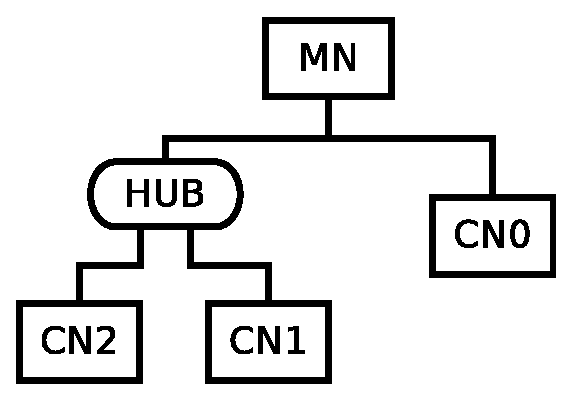
\includegraphics[width=0.5\linewidth]{powerlink_network}
    \caption{POWERLINK network consisting of a \emph{MN} connected to one \emph{CN} and a Ethernet HUB which is connected to two more \emph{CNs}.}
    \label{fig:powerlink_network}
\end{figure}

POWERLINK is based on the standard IEEE 802.3 MAC layer and therefore the usage of default Ethernet hardware is possible.
The different nodes can be arranged in various topologies.
Recommended is the integration of Ethernet HUBs into each node for allowing an easy setup of common used network structures, e.g. a star topology with lines of multiple nodes. \cite[chapter 3]{epsg_epsg_2013}

\subsection{Frame}
\label{sec:oplk_powerlink_frame}
The POWERLINK frame is embedded in the payload of an Ethernet 2 frame and is defined via the Ether type 0x88AB.
Therefore the POWERLINK frame is preceded by the Ethernet 2 Header containing destination \emph{MAC} Address, source \emph{MAC} Address and Ether type.
The payload of an Ethernet 2 Frame can reach up to a length of 1500 bytes succeeding with 4 bytes checksum. \cite[section 3.2]{ethernet_ieee_2016} \cite[section 4.6.1]{epsg_epsg_2013}

In figure \ref{fig:powerlink_frame} the structure of a POWERLINK frame is shown.
The POWERLINK header shown to the left contains the destination and source Node Id preceded by the message type.
The payloads length and content is depending on the transmitted message and thereby defined by the message type. \cite[section 4.6.1.1]{epsg_epsg_2013}

\begin{figure}
    \centering
    \includegraphics[width=0.9\linewidth]{powerlink_frame}
    \caption{POWERLINK frame showing POWERLINK header and payload.}
    \label{fig:powerlink_frame}
\end{figure}

Detailed information about the different structures of transmitted payloads depending on the message type can be found here \cite[section 4.6.1.1.1]{epsg_epsg_2013}

\subsection{Commands}
\label{sec:oplk_powerlink_commands}

As mentioned above different transmitted POWERLINK messages are defined via the message type.
The following commands are distinguished by the according message type.

\begin{description}
    \item[Soc] Start of cycle is sent by the \emph{MN} as multicast and defines the start of the POWERLINK cycle and the isochronous phase.
    \item[PReq] Poll request is sent by the \emph{MN} to a specific \emph{CN} transmitting data and requesting the transmission data from the \emph{CN}.
    \item[PRes] Poll response is sent by the \emph{CN} as multicast as response to a \emph{PReq} and contains data from the \emph{CN}.
    \item[SoA] Start of Asynchronous is sent by the \emph{MN} as multicast and defines the end of the isochronous phase and the begin of the asynchronous phase.
    Additionally the \emph{SoA} message contains the information about the assignment of the following asynchronous slot.
    \item[ASnd] Asynchronous send is sent either by the \emph{MN} or a \emph{CN} as multicast and contains asynchronous data.
\end{description}

The transmission of an \emph{ASnd} message is happening in the asynchronous phase, as described in the next section.
\emph{Asnd} messages can embody different services which are shown in the following listing.\cite[section 4.6.1.1.6.1]{epsg_epsg_2013}

\begin{description}
    \item[IdentResponse] represents a response to a received \emph{IdentRequest}.
    \item[StatusResponse] represents a response to a received \emph{StatusRequest}.
    \item[NMTRequest] represents a response to a received \emph{NMTRequestInvite} when a \emph{NMT} request is pending at the local node.
    \item[NMTCommand] represents a response to a received \emph{NMTRequestInvite} when a \emph{NMT} command is pending at the local node.
    \item[SDO] represents a response to a received \emph{UnspecifiedInvite} and signals an included \emph{SDO} transmission.
    \item[Manufacturer specific] represents manufacturer specific services and usages.
\end{description}

This transmissions are invoked by the preceding \emph{SoA}, which includes an request service id.
According to this request service id the scheduled node is responding with the according response.
The possible requested service ids are shown in the following listing. \cite[section 4.6.1.1.5.1]{epsg_epsg_2013}

\begin{description}
    \item[NoService] indicates that the following asynchronous slot is unassigned.
    \item[IdentRequest] represents an identification query and is used for checking the activity and accessibility of nodes within the POWERLINK network.
    \item[StatusRequest] represents a query of information about a node and its status.
    \item[NMTRequestInvite] represents the assignment message for a pending \emph{NMTCommand} or \emph{NMTRequest}.
    \item[Manufacturer specific] represents manufacturer specific services and usages.
    \item[UnspecifiedInvite] represents the assignment of asynchronous slot for sending any kind of POWERLINK \emph{ASnd} or legacy Ethernet frame.
\end{description}

The sequence of sent commands within a POWERLINK cycle is shown in the next section.

\subsection{Communication cycle}
\label{sec:oplk_powerlink_commcycle}

The POWERLINK communication cycle is separated in two different phases.

The isochronous phase is the first part of a POWERLINK cycle and is started by the \emph{MN} sending a \emph{SoC} message.
Within this phase the \emph{MN} is polling each \emph{CN} with registered isochronous data.
This polling is accomplished by sending a \emph{PReq} message to each \emph{CN}.
This message includes information for the \emph{CN} and also isochronous data which should be sent from the \emph{MN} to the specific \emph{CN}.
After the reception of the \emph{PReq} message the \emph{CN} is sending a \emph{PRes} message as multicast.
This message includes all isochronous data which is requested by the \emph{MN} or any other \emph{CN}.
By multicasting this message each node which should receive a specific data set is immediately receiving the new values. \cite[section 4.2.4.1.1]{epsg_epsg_2013}

When the last isochronous \emph{CN} sent its \emph{PRes} message the isochronous phase is over.
The end of this phase and the start of the asynchronous phase is marked by the sent \emph{SoA} message by the \emph{MN}.
This message contains information about the node which is assigned to the current asynchronous slot.
In each cycle the \emph{MN} assigns the asynchronous slot to either itself or to a \emph{CN}.
Additionally to the assigned node a request service id is transmitted requesting a specific service as described in section \ref{sec:oplk_powerlink_commands}.
Demands a \emph{CN} the assignment to a asynchronous slot this must be communicated to the \emph{MN} either by the \emph{PRes}, \emph{IdentResponse} or \emph{StatusResponse} message.
The communicated number of pending asynchronous messages can additionally provide a priority for better scheduling.
The messages sent within the asynchronous phase can either be an legacy Ethernet frame or an ASnd POWERLINK frame. \cite[section 4.2.4.1.2]{epsg_epsg_2013}

In figure \ref{fig:powerlink_cycle} a simple POWERLINK communication cycle is shown.
Above the horizontal time axis all commands sent by the \emph{MN} are shown.
Commands sent by different \emph{CNs} are displayed below the axis.
This communication cycle shows the isochronous phase marked by the dotted box to the left.
This phase includes the starting command \emph{SoC} and the sequential polling of each \emph{CN}.
This example matches the shown network in figure \ref{fig:powerlink_network} and contains three \emph{CNs}.
The different \emph{CNs} are immediately responding to the polling request.

At the right side in figure \ref{fig:powerlink_cycle} the asynchronous phase is marked by the dashed box.
The asynchronous phase contains the \emph{SoA} command  and following asynchronous data transmission.

\begin{figure}
    \centering
    \includegraphics[width=0.95\linewidth]{powerlink_cycle}
    \caption{POWERLINK communication cylce containing Isochronous Phase with polling of three \emph{CNs} and Asynchronous Phase.}
    \label{fig:powerlink_cycle}
\end{figure}

The transmitted data within isochronous and asynchronous phase and the underlying object model are described in the following section.

\subsection{Data transmission}
\label{sec:oplk_powerlink_data_transmission}
The transmitted data objects are separated in two different groups.

The process data objects (\emph{PDO}) represent time critical data which is transmitted with each cycle.
This transmissions happens during the isochronous phase in the POWERLINK cycle and is enclosed in the \emph{Preq} and \emph{Pres} messages.

When the data of a \emph{PDO} is sent to other nodes it represents a transmit process data object (\emph{TPDO}).
Similar when the received data are stored in a \emph{PDO} this represents a receive process data object (\emph{RPDO}).

The implemented application defines the number of supported \emph{TPDOs} and \emph{RPDOs}, but those are limited to 256 for each type. \cite[section 6.4]{epsg_epsg_2013}
\\

The counterpart to the isochronous transmitted \emph{PDOs} are the service data objects \emph{SDOs}.
\emph{SDOs} provide access to an object within the \emph{OD} of any node within the POWERLINK network.
This access is follows the client-server principle, i.e. the \emph{SDO} client requests the value of an object located inside of the object dictionary (\emph{OD}) of the server.
After receiving the request, the \emph{SDO} server replies with the according data set.
The transmission of these data and the according commands are located within in the asynchronous phase of the POWERLINK cycle.
The granting of sending an asynchronous command is done by the \emph{MN}.

Different functions for accessing the \emph{OD} of the \emph{SDO} server are provided.
More information about the concrete functions for reading and writing a \emph{SDO} can be found in \cite[section 6.3.2.4.2]{epsg_epsg_2013};
\\

The mentioned \emph{OD} contains the definitions of all accessible objects within a POWERLINK network and is described in the next section.

\subsection{Object Dictionary}
\label{sec:oplk_powerlink_object_dictionary}
The \emph{OD} represents a collection of all defined objects which are transmitted via \emph{PDO} or \emph{SOD}, their types and additional communication objects.
Within the \emph{OD} every object is structured in the same way and can represent either a variable, an array or a record of multiple variables.
An object of type array or record contains multiple sub objects which must be of type variable.
Within the \emph{OD} different regions contains definitions for different types and various profiles. \cite[section 2.2.2]{epsg_epsg_2013}

Each object defined in the \emph{OD} consists of the following associated values.

\begin{description}
    \item[Index] represents an identifier of the object within the \emph{OD}.
    \item[Name] is the name of the object.
    \item[Object type] represents the type of the object (variable, array, record).
    \item[Data type] defines the type of the contained data.
    \item[Value range] defines an allowed value range for this object.
    \item[Access] defines the allowed access functions for this object.
    \item[PDO mapping] defines the available mapping possibilities to an \emph{PDO}.
    \item[Default value] defines the value of an uninitialized object.
    \item[Actual value] represents the current value of the object.
\end{description}

More information about the different associated values and further information to the definitions of the \emph{Access} and \emph{PDO mapping} field can be found in \cite{openpowerlink_od_object}.
\\

The openPOWERLINK stack implements the above described functionalities of POWERLINK.
Different demo applications, drivers and the stack implementations are contained in the openPOWERLINK stack distribution.
An introduction in the structure of the stack is given in the following section.


\section{Structure of the openPOWERLINK stack}
\label{sec:oplk_structure}
The openPOWERLINK stack distribution package is structured in different main directories containing demo applications, documentation, driver implementation, stack sources and many more.

For this paper the most important parts are the stack sources and demo applications.
Furthermore an additional simulation directory will be added whose content will be discussed in section \ref{sec:porting_simstub_sim}.

The \emph{apps} folder contains different demo application for embedded targets, linux and windows operating systems.
These demo applications contain exemplary implementations of \emph{MNs} and \emph{CNs}.
These application are analyzed for the development of demo applications within OMNeT++, as described in the section \ref{sec:porting_demo}.

The stack folder contains the following structure. \cite[Directory Structure]{openpowerlink_doc}
\begin{description}
    \item[build] represents the build directory for output files of the build process.
    \item[cmake] contains configuration files for the build tool chain.
    \item[include/oplk] represents the main include directories for all applications using the openPOWERLINK stack.
    \item[include/common] represents a common internal include directory.
    \item[include/kernel] represents an internal include directory for kernel modules.W
    \item[include/target] represents an internal include directory with target specific files.
    \item[include/user] represents an internal include directory for user modules.
    \item[lib] represents the installation directory for the openPOWERLINK libraries.
    \item[proj] represents the directory containing different library projects.
    \item[src/arch] represents a source directory with architecture specific functions.
    \item[src/common] represents a source directory with sources for user and kernel layer.
    \item[src/user] represents a source directory with sources for the user layer.
    \item[src/kernel] represents a source directory with sources for the kernel layer.
\end{description}

This structure represents the architecture of the openPOWERLINK stack, which is explained in the following section.

\section{Architecture}
\label{sec:oplk_architecture}

The openPOWERLINK stack is generally separated in kernel and user layer.
This separation was introduced with the version 2.X of the openPOWERLINK stack and is detaching the higher level user functionalities from the lower level kernel functions including time critical behavior and hardware drivers.
This separation of high level functionalities and time critical procedures allows a real-time communication independent of the running application and the executed user functions.

The separation of kernel and user layer using the communication abstraction layer (\emph{CAL}) is shown in figure \ref{fig:openpowerlink_arch}.

\begin{figure}
\centering
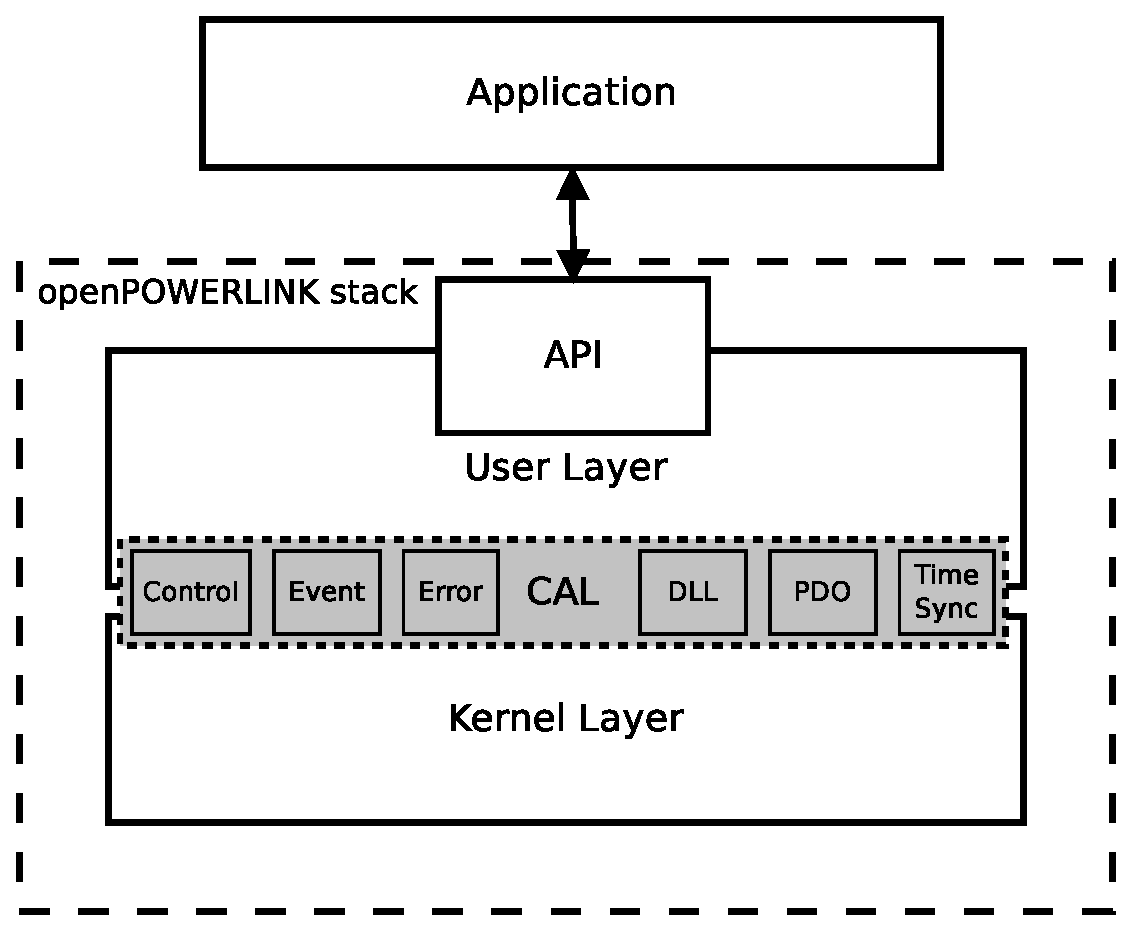
\includegraphics[width=0.9\linewidth]{images/openpowerlink_arch}
\caption{Software architecture of the openPOWERLINK stack.}
\label{fig:openpowerlink_arch}
\end{figure}


\subsection{Kernel layer}
\label{sec:oplk_architecture_kernel}

The kernel layer of the openPOWERLINK stack contains the following modules. \cite[openPOWERLINK Kernel Layer]{openpowerlink_doc}

\begin{description}
    \item[Control module] manages shutdown and startup commands for the kernel stack.
    \item[Data link layer (\emph{DLL}] implements the \emph{DLL} state machine and handles the creating and processing of the POWERLINK cycle.
    \item[Error handler] implements the POWERLINK error handler and manages the error counters.
    \item[Event handler] provides functionalities for posting events to other kernel modules and to the user layer.
    This handler also processes events posted by the user layer.
    \item[Led module] controls the POWERLINK status and error Leds.
    \item[\emph{PDO} module] handles the \emph{PDOs} in the openPOWERLINK kernel layer and communicates with the \emph{DLL} module for the transmission of the \emph{PDO}s.
    \item[Network management (\emph{NMT} module)] implements the \emph{NMT} state machine and provides the general functions for network management.
    \item[Virtual Ethernet driver] provides a network interface for sending Ethernet packets.
    These packets will be transmitted during the asynchronous phase.
    \item[High resolution timer module] provides high resolution timer functionalities for timing the POWERLINK cycle.
    \item[Synchronization timer module] implements the synchronization of a \emph{CN} to the POWERLINK cycle.
    \item[Timestamp module] provides helper functions for handling of timestamps.
    \item[Time synchronization module] implements the time synchronization to the POWERLINK network.
\end{description}

Running on an operating system, e.g. linux, the kernel layer can be built and executed separately as a kernel module of the operating system.
Such a communication mode is defined via the configurations of the different stack projects (proj folder).
The configurations are affecting the communication abstraction layer \emph{CAL} described in section \ref{sec:oplk_architecture_cal}.

\subsection{User layer}
\label{sec:oplk_architecture_user}

The user layer includes higher level functions and provides the application programming interface (\emph{API}) for an application using the openPOWERLINK stack.
The following modules are located within the user layer. \cite[openPOWERLINK User Layer]{openpowerlink_doc}

\begin{description}
    \item[API] represents the interface to the application and provides all functions for interactions with the openPOWERLINK stack.
    \item[Control module] manages shutdown and startup commands for the user stack.
    \item[Error handler] handles the synchronization of error counters located in the kernel layer with the according objects in the \emph{OD}.
    \item[Event handler] provides functionalities for posting events to other user modules and to the kernel layer.
    This handler also processes events posted by the kernel layer.
    \item[\emph{PDO} module] handles exchanging of process image data via the process image \emph{API}.
    \item[\emph{SDO} modules] provide the \emph{SDO} stack of openPOWERLINK including command layer, sequence layer and the transmission implementation using \emph{ASnd} or \emph{UDP}.
    \item[Network management (\emph{NMT} modules)] implements various \emph{NMT} functions of the user layer including functions for \emph{MN} and \emph{CN} and the handling of the \emph{Ident}-, \emph{Status}- and \emph{Sync}-requests.
    \item[Configuration manager module] implements the handling of the \emph{CDC} file and the configuration of connected \emph{CNs} using \emph{SDO} transmission.
    \item[\emph{OD} module] implements the POWERLINK \emph{OD}.
    \item[\emph{OD} abstraction layer] provides an abstraction layer for accessing different POWERLINK \emph{ODs}.
    \item[Timer module] implements timer functionalities used by the user stack modules.
    \item[Time synchronization module] provides a configurable notification at a specific synchronization point for the application.
\end{description}

\subsection{Communication abstraction Layer}
\label{sec:oplk_architecture_cal}

The user and kernel layer are separated by the communication abstraction layer (\emph{CAL}).
This layer is separated in different modules for each module within kernel and user layer which must communicate with the opposite module.
The separation of the \emph{CAL} and placement between the kernel and user layer is shown in figure \ref{fig:openpowerlink_arch}.
The gray dotted box shows the \emph{CAL} and all embedded modules using a \emph{CAL} related implementation.

The following modules use \emph{CAL} modules for communication between kernel and user layer. 

\begin{itemize}
    \item control module
    \item event handler
    \item error handler
    \item data link layer (\emph{DLL})
    \item process data objects (\emph{PDO})
    \item time sync
\end{itemize}

For the listed modules two \emph{CAL} modules are necessary within user and kernel layer.
Using a specific \emph{CAL} implementation must be configured in both layers.
Different implementations of the \emph{CAL} modules allow various configurations and compositions of the openPOWERLINK stack using different communication methods between kernel and user layer. \cite[CAL]{openpowerlink_doc}

\subsection{Hardware abstraction}
\label{sec:oplk_architecture_hardware}
The openPOWERLINK stack implements the support of different operating systems and hardware platforms by definition of the modules functions in a common header.
The compiled implementation represents the specification for each platform.

The platform dependency of the openPOWERLINK stack and the platform dependent modules are analyzed in section \ref{sec:oplk_platform}.

The dependency of the platform regarding byte endianess is handled by the abstract memory interface described in the next section.

\subsection{Abstract memory interface}
\label{sec:oplk_architecture_ami}

The abstract memory interface (\emph{AMI}) provides multiple simple functions for the correct handling of data fields affected by the byte endianess.
Similar to the \emph{CAL} and hardware abstraction the implementations for different platforms are defined by compiling the according implementation. \cite[AMI]{openpowerlink_doc}
\\

The openPOWERLINK stack provides multiple configurable implementation and communication variants.
These are manages within the used tool chain described in the next section.

\section{Configuration and build}
\label{sec:oplk_build}
For configuration and building of the openPOWERLINK stack the built tool \emph{CMAKE} is used.
The main \emph{CMAKE} file \emph{CMakeLists.txt} checks the current \emph{CMAKE\_SYSTEM\_NAME} variable and uses the according configuration matching the targeted platform.

The global \emph{CMAKE} file loads according to the \emph{CMAKE\_SYSTEM\_NAME} and \emph{CMAKE\_SYSTEM\_PROCESSOR} variable the correct system specific options file.
This option file includes options for enabling and disabling part of the openPOWERLINK stack.
For example the generation of the \emph{CN} or \emph{MN} library can be en- or disabled.
Further options are platform specific and provide configuration possibilities for various features available in different implementations and on different platforms.

Requires the targeted platform a custom tool chain so a specific tool chain file must be defined containing configurations regarding the used tool chain.

The \emph{CAL}, hardware abstraction and \emph{AMI} are using specific implementations of common header files.
These sets of specific sources are defined within the common \emph{CMAKE} file \emph{stackfiles.cmake}.
This file includes groups defined source files for each module and each implementation specialization.
The usage of such specific groups is done in project specific \emph{CMAKE} files composing various stack variants for specific platforms. \cite[Building openPOWERLINK]{openpowerlink_doc}

Within the system specific options file all defined projects matching this system are included in the configuration.
These projects are located in the \emph{proj} folder as described in the following section.

\subsection{Library projects} %TODO rework
\label{sec:oplk_structure_proj}
Located in the \emph{proj} folder various projects for different systems are defined.
These projects are grouped in the following systems.

\begin{description}
    \item[generic] contains projects for embedded targets without underlying operating systems.
    \item[linux] contains projects for linux operating systems.
    \item[windows] contains projects for windows operating systems.
\end{description}

Within each system specific folder different projects are located.
These different projects use different features and functionalities of the openPOWERLINK stack.
Within the different project directories the \emph{CMakeLists.txt} file defines the used implementations and sources.
The groups defined in the \emph{stackfiles.cmake} file are used and combined within the project specific \emph{CMAKE} file.

Additional configurations made by preprocessor defines are set in the \emph{oplkcfg.h} header file within each project directory.
\\

Executing the \emph{CMAKE} build tool generates the according makefile.
Using this makefile either all included or specific projects can be built and installed at a defined install directory.

\section{Platform dependency}
\label{sec:oplk_platform}
%TODO: rework and enhance
As described in section \ref{sec:oplk_structure} the configuration and build process defines the according platform specific implementations and libraries.

For platform specific functionalities the implementation of the openPOWERLINK stack uses common header files with specific implementations.

For defining which implementations are platform specific the \emph{CMAKE} file \emph{stackfile.cmake} is analyzed.

The following modules are implemented platform dependent:

\begin{description}
    \item[oplkinc.h] provides macros for target specific functions which depends on the targeting platform or operating systems.
    Defined are small standard functions regarding memory operations.
    \item[Trace] module providing a function for tracing the execution.
    \item[\emph{OBD} configuration] containing specific for functions for storing and restoring of the \emph{OD}.
    The implementation is split in functions regarding file operations and a generic cyclic redundancy check (\emph{CRC}) calculation.
    \item[\emph{SDO} via \emph{UDP}] this implementation contains the transmission of \emph{SDO}s via user datagram protocol (\emph{UDP}).
    The specific implementations provide usage of operating system calls of linux and windows or the usage of a generic header \emph{socketwrapper.h} which allows the implementation for other targets.
    \item[\emph{CAL}] includes different interfaces for the user and kernel space for each containing module (control, \emph{DLL}, \emph{PDO}, error handler, event).
    \item[Timer] providing functions for setting timer.
    \item[Circular buffer] providing the system specific functionalities used within the \emph{circular\_buffer} as creation, allocation, deallocation, locking, connecting and disconnecting.
    \item[Memmap] providing an interface for the memory mapping library used for memory mapped communication in between kernel and user space.
    \item[Target] providing an interface for target specific functions as sleep, interrupt control, tick and implementations of locks and mutexes.
    \item[\emph{AMI}] providing an interface for architecture specific memory functions.
    \item[Edrv] represents the Ethernet driver which is communicating with the used Ethernet media access control (\emph{MAC}) controller.
\end{description}

The porting ot the described platform dependencies to the OMNeT++ simulation environment and the according analyzes are described in the following chapter.
\chapter{Simulation of openPOWERLINK}
\label{cha:porting}

As described in section \ref{sec:oplk_platform} multiple modules contain platform specific functionalities.
The openPOWERLINK stack can be built with various configurations, depending on the settings and the compositions configured individually more or less platform specific modules are used.
These configurations are defined within the different projects in the \emph{proj} folder, as explained in section \ref{sec:oplk_structure_proj}.

\section{Analyze of existing projects}
\label{cha:porting_projects}

\subsection{liboplkmn}
\label{cha:porting_projects_liboplkmn}

The \emph{liboplkmn} represents a \emph{MN} library consisting of a single library including the user and kernel space.
Analyzing the \emph{liboplkmn} for linux results in following modules which must be ported:

\begin{itemize}
    \item Target
    \item \emph{SDO} via \emph{UDP}
    \item Trace
    \item Timer
    \item CircularBuffer
\end{itemize}

The first step for the implementation of the \emph{MN} library for OMNeT++ is the integration in the configuration and build process within the openPOWERLINK stack.
Therefore an according options file and toolchain file for integration in the \emph{CMAKE} process are created.
\chapter{Results}
\label{cha:results}

\section{Simulated network}
\label{sec:results_network}
The implemented network for simulating a POWERLINK network consists of a \emph{MN} module connected to a single \emph{CN} module.
This network is shown in figure \ref{fig:results_mn_single_cn};

\begin{figure}
    \centering
    %\includegraphics[width=0.9\linewidth]{}
    \caption{Simulated network consisting of a \emph{MN} module directly connected to a \emph{MN} module.}
    \label{fig:results_mn_single_cn}
\end{figure}

\chapter{Conclusion}
\label{cha:conclusion}

\section{Future Simulations}
\label{sec:conclusion_futuresim}
\begin{sloppypar}
The developed OMNeT++ modules allow the simulation of a simple \mbox{POWERLINK} network consisting of an openPOWERLINK \emph{MN} and a \emph{CN}.
This simulation was developed for optimal performance using a monolithic design.
Alternative simulations can be implemented based on the basic strategies and reusable functionalities represented by the developed base classes, helper classes and interfaces.
For a deeper insight, a modular design could be implemented by connecting the \emph{CAL} modules with the simulation.
This could be done in a similar way as handling the platform dependency by implementing according simulation specific modules redirecting the communicated calls and data into the simulation environment.
Within the simulation environment even both modules of a \emph{CAL} component could be modeled separately.
This would lead to the encapsulation of the communicated data in messages.
Such an implementation of \emph{CAL} components within OMNeT++ would allow for deeper insights into the openPOWERLINK stack and the communication between kernel and user layer.
\end{sloppypar}

The simulated network contains a direct connection between the different nodes.
This represents an optimal behavior and results in an ideal performance.
For simulating the behavior of openPOWERLINK nodes in a network including real devices this connection would have to be changed.
Existing functionality from the INET library regarding Ethernet and UDP could be used for converting the transmitted messages to real Ethernet frames.

\section{Future Development}
\label{sec:conclusion_futuredev}
The development of the resulting simulation and the according implementations will continue to allow developers an easy access to openPOWERLINK.
This easy access should be provided by a flexible simulation environment with different levels of modularity and complexity.
Such an environment will provide deep insight in the openPOWERLINK stack and an possible overview for bigger networks consisting of various topologies and nodes.

This simulation environment will be developed as Open Source project and thereby made available for every interested developer.

\section{Emulation}
\label{sec:conclusion_emulation}
The simulation mode of real-time simulation and the possibilities for emulation using OMNeT++  show a good starting point for the customized development of such applications.
The built-in functionality and its usage within the examples (\emph{sockets}) reflect the basic strategies for developing an emulation.
This functionality should be used as a basis for developing more optimized and customized functionalities.

\section{Experiences}
\label{sec:conclusion_experiences}
The built-in functionalities and the corresponding possibilities of OMNeT++ are extensive.
This large number of configurations and components can cause a difficult approach to the developing of a simulation.
But investing more time in exploring OMNeT++ pays off well, because of the flexibility and the various fields of possible applications.

\section{Outlook}
\label{sec:conclusion_outlook}
The fields of simulation, emulation and \emph{HiL} are steadily gaining importance owing to the growing requirement for comprehensive testing.
OMNeT++ represents a dynamic framework for various applications and a high order of flexibility.
This allows for the development of simulations for various fields.

The connection between simulations using OMNeT++ with embedded systems portrays a promising avenue to pursue in terms of testing and developing new systems.

%%%----------------------------------------------------------
%%%Anhang
\appendix
\chapter{OMNeT++ Code Snippets}
\label{app:omnetpp_code}

\section{cRealTimeScheduler}
\label{app:omnetpp_code_real_time_scheduler}

\lstinputlisting[caption=Definition of \emph{cRealTimeScheduler},firstnumber=138,firstline=138,lastline=200]{\omnetpproot/include/cscheduler.h}
\lstinputlisting[caption=Implementation of \emph{cRealTimeScheduler},firstnumber=63,firstline=63,lastline=133]{\omnetpproot/src/sim/cscheduler.cc}

\section{sockets Sample}
\label{app:omnetpp_code_socket}


\subsection{SocketRTScheduler}
\label{app:omnetpp_code_socket_scheduler}

\lstinputlisting[caption=Definition of \emph{SocketRTScheduler}]{\omnetpproot/samples/sockets/SocketRTScheduler.h}
\lstinputlisting[caption=Implementation of \emph{SocketRTScheduler}]{\omnetpproot/samples/sockets/SocketRTScheduler.cc}

\subsection{ExtHttpClient}
\label{app:omnetpp_code_socket_http}

\lstinputlisting[caption=Implementation of \emph{ExtHttpClient}]{\omnetpproot/samples/sockets/ExtHttpClient.cc}

\subsection{ExtTelnetClient}
\label{app:omnetpp_code_socket_telnet}

\lstinputlisting[caption=Implementation of \emph{ExtTelnetClient}]{\omnetpproot/samples/sockets/ExtTelnetClient.cc}


% placement settings for following figures
%\floatplacement{figure}{H}

\chapter{Further design Measurements}
\label{app:measurements}

This chapter includes all plots of analyzed design measurements executed on the additional host machines.

\section{Workstation measurements}
\label{app:measurements_workstation}

\subsection{Runtime}
\label{app:measurements_workstation_runtime}

% runtime over simtime
\begin{figure} [H]
    \centering
    \pgfplotsset{
        every axis plot/.append style={very thick}
    }
    \begin{tikzpicture}
    \begin{axis}[
    xmode=log,
    ymode=log,
    ylabel={Runtime [s]},
    xlabel={Simulation time [s]},
    grid=major,
    legend entries={Modular,Monolithic},
    legend style={at={(0.03,0.97)}, anchor=north west}
    ]
    
    \addplot table {../results/workstation/runtimeResults.Modular.txt};
    \addplot table {../results/workstation/runtimeResults.Monolithic.txt};
    \end{axis}
    \end{tikzpicture}    
    \caption{Runtime results for different designs over a varying simulation time.}
    \label{fig:app_workstation_runtime_simtime}
\end{figure}

%%% runtime over number of event manager %%%
\begin{figure} [H]
    \centering
    \pgfplotsset{
        every axis plot/.append style={very thick}
    }
    \begin{tikzpicture}
    \begin{axis}[
    xmode=log,
    %ymode=log,
    ylabel={Runtime [s]},
    xlabel={Number of \emph{EventManager}},
    grid=major,
    legend entries={Modular,Monolithic},
    legend style={at={(0.97,0.5)},anchor=east}
    ]
    
    \addplot table {../results/workstation/runtime/simtimeEventManagerResults.Modular.txt};
    \addplot table {../results/workstation/runtime/simtimeEventManagerResults.Monolithic.txt};
    \end{axis}
    \end{tikzpicture}    
    \caption{Runtime using different designs over variing number of \emph{EventManager}.}
    \label{fig:app_workstation_runtime_eventmanagers}
\end{figure}


%%% runtime over polling interval %%%
\begin{figure} [H]
    \centering
    \pgfplotsset{
        every axis plot/.append style={very thick}
    }
    \begin{tikzpicture}
    \begin{axis}[
    xmode=log,
    ymode=log,
    ylabel={Runtime [s]},
    xlabel={Polling interval [ns]},
    grid=major,
    legend entries={Modular,Monolithic},
    legend style={at={(0.97,0.97)}, anchor=north east}
    ]
    
    \addplot table {../results/workstation/runtime/simtimePollingResults.Modular.txt};
    \addplot table {../results/workstation/runtime/simtimePollingResults.Monolithic.txt};
    \end{axis}
    \end{tikzpicture}    
    \caption{Runtime using different designs over varying polling interval by the \emph{HistoryManager}.}
    \label{fig:app_workstation_runtime_polling}
\end{figure}


%%% runtime over generation interval %%%
\begin{figure} [H]
    \centering
    \pgfplotsset{
        every axis plot/.append style={very thick}
    }
    \begin{tikzpicture}
    \begin{axis}[
    xmode=log,
    ymode=log,
    ylabel={Runtime [s]},
    xlabel={Generation interval [ns]},
    grid=major,
    legend entries={Modular,Monolithic},
    legend style={at={(0.97,0.97)}, anchor=north east}
    ]
    
    \addplot table {../results/workstation/runtime/simtimeGenerationResults.Modular.txt};
    \addplot table {../results/workstation/runtime/simtimeGenerationResults.Monolithic.txt};
    \end{axis}
    \end{tikzpicture}    
    \caption{Runtime using different designs over varying generation interval by the \emph{Generator}.}
    \label{fig:app_workstation_runtime_generation}
\end{figure}

\subsection{Event}
\label{app:measurements_workstation_event}

%%% event number over cpu time %%%
\begin{figure} [H]
    \centering
    \pgfplotsset{
        every axis plot/.append style={very thick}
    }
    \begin{tikzpicture}
    \begin{axis}[
    xmode=log,
    ymode=log,
    ylabel={Created event},
    xlabel={Cpu time $[s]$},
    grid=major,
    legend entries={Modular,Monolithic},
    legend style={at={(0.03,0.97)}, anchor=north west}
    ]
    
    \addplot table {../results/workstation/eventResults.Modular.txt};
    \addplot table {../results/workstation/eventResults.Monolithic.txt};
    \end{axis}
    \end{tikzpicture}    
    \caption{Created events for different designs over different cpu time limits.}
    \label{fig:app_workstation_event_cputime}
\end{figure}

%%% events over Event managers %%%
\begin{figure} [H]
    \centering
    \pgfplotsset{
        every axis plot/.append style={very thick}
    }
    \begin{tikzpicture}
    \begin{axis}[
    xmode=log,
    %ymode=log,
    ylabel={Created events},
    xlabel={Number of EventManager},
    grid=major,
    legend entries={Modular,Monolithic},
    legend style={at={(0.97,0.5)},anchor=east}
    ]
    
    \addplot table {../results/workstation/event/cputimeEventManagerResults.Modular.txt};
    \addplot table {../results/workstation/event/cputimeEventManagerResults.Monolithic.txt};
    \end{axis}
    \end{tikzpicture}    
    \caption{Created events using different designs over varying number of \emph{EventManager}.}
    \label{fig:app_workstation_event_eventmanagers}
\end{figure}

%%% events over polling interval %%%
\begin{figure} [H]
    \centering
    \pgfplotsset{
        every axis plot/.append style={very thick}
    }
    \begin{tikzpicture}
    \begin{axis}[
    xmode=log,
    ymode=log,
    ylabel={Created events},
    xlabel={Polling interval [ns]},
    grid=major,
    legend entries={Modular,Monolithic},
    legend style={at={(0.03,0.5)},anchor=west}
    ]
    
    \addplot table {../results/workstation/event/cputimePollingResults.Modular.txt};
    \addplot table {../results/workstation/event/cputimePollingResults.Monolithic.txt};
    \end{axis}
    \end{tikzpicture}    
    \caption{Created events using different designs over varying polling interval by the \emph{HistoryManager}.}
    \label{fig:app_workstation_event_polling}
\end{figure}

\section{Build server measurements}
\label{app:measurements_build_server}

\subsection{Runtime}
\label{app:measurements_build_server_runtime}

% runtime over simtime
\begin{figure} [H]
    \centering
    \pgfplotsset{
        every axis plot/.append style={very thick}
    }
    \begin{tikzpicture}
    \begin{axis}[
    xmode=log,
    ymode=log,
    ylabel={Runtime [s]},
    xlabel={Simulation time [s]},
    grid=major,
    legend entries={Modular,Monolithic},
    legend style={at={(0.03,0.97)}, anchor=north west}
    ]
    
    \addplot table {../results/buildServer/runtimeResults.Modular.txt};
    \addplot table {../results/buildServer/runtimeResults.Monolithic.txt};
    \end{axis}
    \end{tikzpicture}    
    \caption{Runtime results for different designs over a varying simulation time.}
    \label{fig:app_build_server_runtime_simtime}
\end{figure}

%%% runtime over number of event manager %%%
\begin{figure} [H]
    \centering
    \pgfplotsset{
        every axis plot/.append style={very thick}
    }
    \begin{tikzpicture}
    \begin{axis}[
    xmode=log,
    %ymode=log,
    ylabel={Runtime [s]},
    xlabel={Number of \emph{EventManager}},
    grid=major,
    legend entries={Modular,Monolithic},
    legend style={at={(0.97,0.5)},anchor=east}
    ]
    
    \addplot table {../results/buildServer/runtime/simtimeEventManagerResults.Modular.txt};
    \addplot table {../results/buildServer/runtime/simtimeEventManagerResults.Monolithic.txt};
    \end{axis}
    \end{tikzpicture}    
    \caption{Runtime using different designs over variing number of \emph{EventManager}.}
    \label{fig:app_build_server_runtime_eventmanagers}
\end{figure}


%%% runtime over polling interval %%%
\begin{figure} [H]
    \centering
    \pgfplotsset{
        every axis plot/.append style={very thick}
    }
    \begin{tikzpicture}
    \begin{axis}[
    xmode=log,
    ymode=log,
    ylabel={Runtime [s]},
    xlabel={Polling interval [ns]},
    grid=major,
    legend entries={Modular,Monolithic},
    legend style={at={(0.97,0.97)}, anchor=north east}
    ]
    
    \addplot table {../results/buildServer/runtime/simtimePollingResults.Modular.txt};
    \addplot table {../results/buildServer/runtime/simtimePollingResults.Monolithic.txt};
    \end{axis}
    \end{tikzpicture}    
    \caption{Runtime using different designs over varying polling interval by the \emph{HistoryManager}.}
    \label{fig:app_build_server_runtime_polling}
\end{figure}


%%% runtime over generation interval %%%
\begin{figure} [H]
    \centering
    \pgfplotsset{
        every axis plot/.append style={very thick}
    }
    \begin{tikzpicture}
    \begin{axis}[
    xmode=log,
    ymode=log,
    ylabel={Runtime [s]},
    xlabel={Generation interval [ns]},
    grid=major,
    legend entries={Modular,Monolithic},
    legend style={at={(0.97,0.97)}, anchor=north east}
    ]
    
    \addplot table {../results/buildServer/runtime/simtimeGenerationResults.Modular.txt};
    \addplot table {../results/buildServer/runtime/simtimeGenerationResults.Monolithic.txt};
    \end{axis}
    \end{tikzpicture}    
    \caption{Runtime using different designs over varying generation interval by the \emph{Generator}.}
    \label{fig:app_build_server_runtime_generation}
\end{figure}


\subsection{Event}
\label{app:measurements_build_server_event}

%%% event number over cpu time %%%
\begin{figure} [H]
    \centering
    \pgfplotsset{
        every axis plot/.append style={very thick}
    }
    \begin{tikzpicture}
    \begin{axis}[
    xmode=log,
    ymode=log,
    ylabel={Created event},
    xlabel={Cpu time $[s]$},
    grid=major,
    legend entries={Modular,Monolithic},
    legend style={at={(0.03,0.97)}, anchor=north west}
    ]
    
    \addplot table {../results/buildServer/eventResults.Modular.txt};
    \addplot table {../results/buildServer/eventResults.Monolithic.txt};
    \end{axis}
    \end{tikzpicture}    
    \caption{Created events for different designs over different cpu time limits.}
    \label{fig:app_build_server_event_cputime}
\end{figure}

%%% events over Event managers %%%
\begin{figure} [H]
    \centering
    \pgfplotsset{
        every axis plot/.append style={very thick}
    }
    \begin{tikzpicture}
    \begin{axis}[
    xmode=log,
    %ymode=log,
    ylabel={Created events},
    xlabel={Number of EventManager},
    grid=major,
    legend entries={Modular,Monolithic},
    legend style={at={(0.97,0.5)},anchor=east}
    ]
    
    \addplot table {../results/buildServer/event/cputimeEventManagerResults.Modular.txt};
    \addplot table {../results/buildServer/event/cputimeEventManagerResults.Monolithic.txt};
    \end{axis}
    \end{tikzpicture}    
    \caption{Created events using different designs over varying number of \emph{EventManager}.}
    \label{fig:app_build_server_event_eventmanagers}
\end{figure}

%%% events over polling interval %%%
\begin{figure} [H]
    \centering
    \pgfplotsset{
        every axis plot/.append style={very thick}
    }
    \begin{tikzpicture}
    \begin{axis}[
    xmode=log,
    ymode=log,
    ylabel={Created events},
    xlabel={Polling interval [ns]},
    grid=major,
    legend entries={Modular,Monolithic},
    legend style={at={(0.97,0.5)},anchor=east}
    ]
    
    \addplot table {../results/buildServer/event/cputimePollingResults.Modular.txt};
    \addplot table {../results/buildServer/event/cputimePollingResults.Monolithic.txt};
    \end{axis}
    \end{tikzpicture}    
    \caption{Created events using different designs over varying polling interval by the \emph{HistoryManager}.}
    \label{fig:app_build_server_event_polling}
\end{figure}

%%% events over generation interval %%%
\begin{figure} [H]
    \centering
    \pgfplotsset{
        every axis plot/.append style={very thick}
    }
    \begin{tikzpicture}
    \begin{axis}[
    xmode=log,
    ymode=log,
    ylabel={Created events},
    xlabel={Generation interval [ns]},
    grid=major,
    legend entries={Modular,Monolithic},
    legend style={at={(0.97,0.5)},anchor=east}
    ]
    
    \addplot table {../results/buildServer/event/cputimeGenerationResults.Modular.txt};
    \addplot table {../results/buildServer/event/cputimeGenerationResults.Monolithic.txt};
    \end{axis}
    \end{tikzpicture}    
    \caption{Created events using different designs over varying generation interval by the \emph{Generator}.}
    \label{fig:app_build_server_event_generation}
\end{figure}

\subsection{Real-time}
\label{app:measurements_build_server_realtime}


% realtime over sim time
\begin{figure} [H]
    \centering
    \pgfplotsset{
        every axis plot/.append style={very thick}
    }
    \begin{tikzpicture}
    \begin{axis}[
    xmode=log,
    ymode=log,
    ylabel={Achievable real time generation interval [ns]},
    xlabel={Simulation time [s]},
    grid=major,
    legend entries={Modular,Monolithic},
    legend style={at={(0.97,0.5)}, anchor=east}
    ]
    
    \addplot table {../results/buildServer/realTimeResults.Modular.txt};
    \addplot table {../results/buildServer/realTimeResults.Monolithic.txt};
    \end{axis}
    \end{tikzpicture}    
    \caption{Real-time results for different designs over different simulation time limits.}
    \label{fig:app_build_server_realtime_simtime}
\end{figure}


% realtime over event managers
\begin{figure} [H]
    \centering
    \pgfplotsset{
        every axis plot/.append style={very thick}
    }
    \begin{tikzpicture}
    \begin{axis}[
    xmode=log,
    ymode=log,
    ylabel={Achievable real time generation interval [ns]},
    xlabel={Number of \emph{Eventmanagers}},
    grid=major,
    legend entries={Modular,Monolithic},
    legend style={at={(0.97,0.5)}, anchor=east}
    ]
    
    \addplot table {../results/buildServer/realtime/rtEventManagerResults.Modular.txt};
    \addplot table {../results/buildServer/realtime/rtEventManagerResults.Monolithic.txt};
    \end{axis}
    \end{tikzpicture}    
    \caption{Real-time results for different designs over a varying number of \emph{EventManagers}.}
    \label{fig:app_build_server_realtime_eventmanager}
\end{figure}


% realtime over polling interval
\begin{figure} [H]
    \centering
    \pgfplotsset{
        every axis plot/.append style={very thick}
    }
    \begin{tikzpicture}
    \begin{axis}[
    xmode=log,
    ymode=log,
    ylabel={Achievable real time generation interval [ns]},
    xlabel={Polling interval of \emph{HistoryManager} [ns]},
    grid=major,
    legend entries={Modular,Monolithic},
    legend style={at={(0.97,0.5)}, anchor=east}
    ]
    
    \addplot table {../results/buildServer/realtime/rtPollingResults.Modular.txt};
    \addplot table {../results/buildServer/realtime/rtPollingResults.Monolithic.txt};
    \end{axis}
    \end{tikzpicture}    
    \caption{Real-time results for different designs over a varying polling interval of \emph{HistoryManager}.}
    \label{fig:app_build_server_realtime_polling}
\end{figure}


%%%----------------------------------------------------------
\MakeBibliography
%%%----------------------------------------------------------

%%%Messbox zur Druckkontrolle
\include{messbox}

\end{document}
